\paragraph{QuizziPedia::Back-End::App::Routers::UserRouter}
\label{QuizziPedia::Back-End::App::Routers::UserRouter}
\begin{figure}[ht]
	\centering
	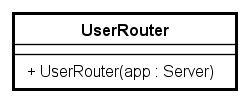
\includegraphics[scale=0.45]{UML/Classi/Back-End/QuizziPedia_Back-End_App_Routers_UserRouter.png}
	\caption{QuizziPedia::Back-End::App::Routers::UserRouter}
\end{figure}
\FloatBarrier
	\begin{itemize}
		\item \textbf{Descrizione} \\
		Classe che gestisce le richieste relative alla registrazione, alla gestione della sessione e alla cronologia dei questionari svolti di un utente.
Componente ConcreteHandler del design pattern \textit{Chain of responsibility\ped{G}}. Utilizza il modulo \textit{Passport\ped{G}}.
		\item \textbf{Utilizzo} \\
		Viene utilizzata per chiamare il controller che si occupa di gestire le API relative alla registrazione, alla gestione della sessione e alla cronologia dei questionari di un utente.
		\item \textbf{Relazioni con altre classi} 
		\begin{itemize}
		\item 
			IN	\texttt{Server}\\
			Classe che avvia il server. Nello specifico apre una connessione al database tramite \textit{Mongoose\ped{G}}, invoca il middleware \textit{Express\ped{G}} passando un riferimento al database MongoDB come parametro in modo che possa configurarsi con esso, invoca il \textit{middleware\ped{G}} \textit{Passport\ped{G}} ed infine si mette in ascolto su una determinata porta. È il componente client del design pattern \textit{Chain of responsibility\ped{G}}. Utilizza i moduli \textit{Mongoose\ped{G}}, \textit{Express\ped{G}}, \textit{Passport\ped{G}}. 
		\item 
			OUT \texttt{ErrorHandler}\\
			Classe \textit{middleware\ped{G}} per la gestione degli errori. Ritorna al client un oggetto di tipo Response con stato \textit{HTTP\ped{G}} 500 e descrizione dell’errore in formato \textit{JSON\ped{G}}. È un
componente ConcreteHandler del design pattern \textit{Chain of responsibility\ped{G}}.
		\item 
			OUT \texttt{NotFoundHandler}\\
			Classe che si occupa della gestione dell’errore di pagina non trovata. Componente ConcreteHandler del design pattern \textit{Chain of responsibility\ped{G}}.
		\item 
			OUT \texttt{UserController}\\
			Classe che raggruppa attraverso require i vari controllers responsabili delle operazioni legate alla gestione degli utenti. Si è scelto di predisporre questo raggruppamento per facilitare l'introduzione di nuove funzionalità legate alla gestione degli utenti.
		\item 
			OUT \texttt{SummaryController}\\
			Classe che gestisce la cronologia dei questionari svolti dall'utente
	\end{itemize}
		\item \textbf{Metodi} 
		\begin{itemize}
		\item 
		\texttt{+ UserRouter(app: Server)} \\
		Contiene diverse route che vengono configurate all’avvio del server. Quest’ultime ricevono le richieste del client e passano il controllo al ConcreteHandler successivo.
		\textbf{Parametri}:
			\begin{itemize}
				\item 
				\texttt{app: Server} \\
				Rappresenta l’istanza del server su cui configurare i route che mappano i controllers specifici.
			\end{itemize}
		\end{itemize}
\end{itemize}		